\section{Computation}

Provide computation methods and data of what I have done so far.

This is how you can refer to fig \ref{fig:liq vap co}. % Note: Have to build the latex document twice for it to work.


%sample image input
\begin{figure}[h]
	\centering
	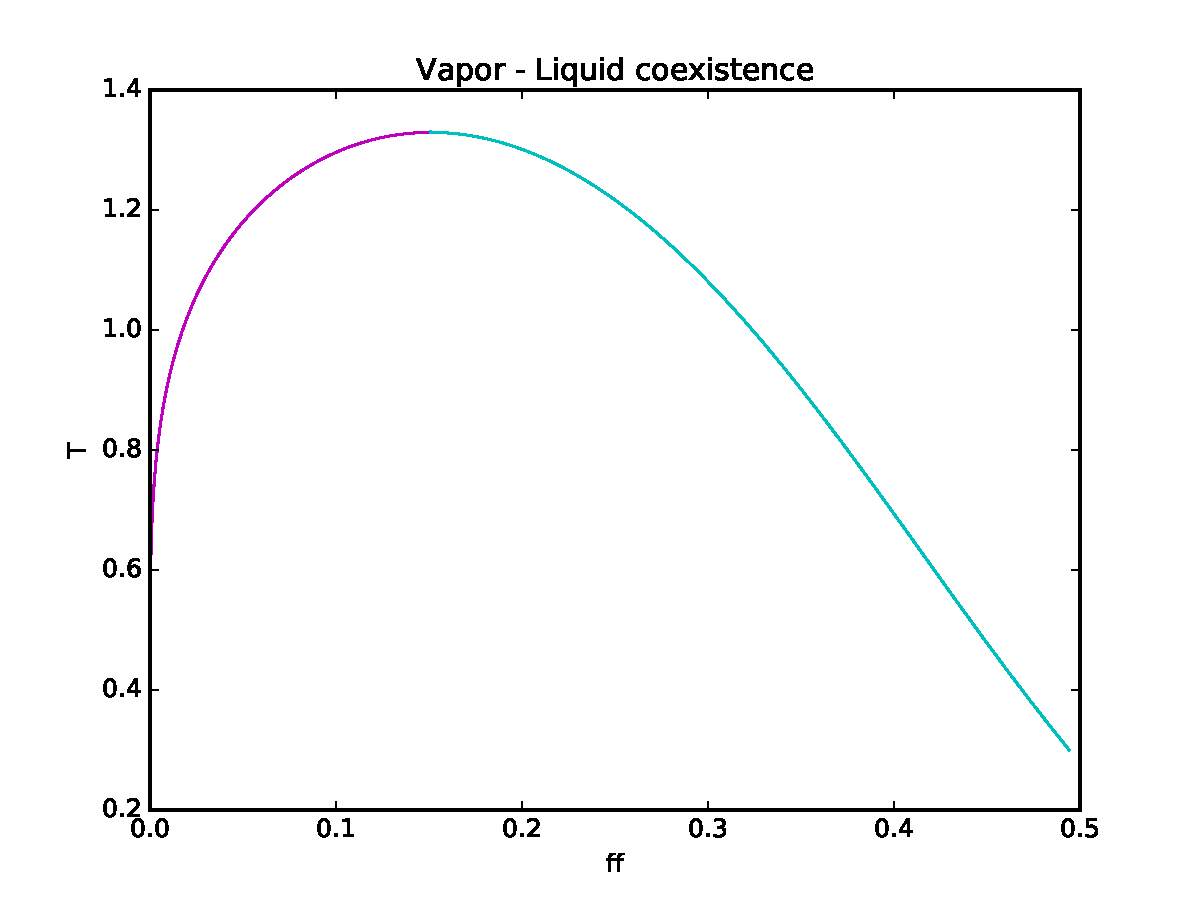
\includegraphics[scale=0.5]{liqVapCo_Tvsff}
	\caption{Caption for this image.}
	\label{fig:liq vap co}
\end{figure}

%sample multi image input
\begin{figure}[h]
	\centering
	\begin{subfigure}[b]{0.3\textwidth}
	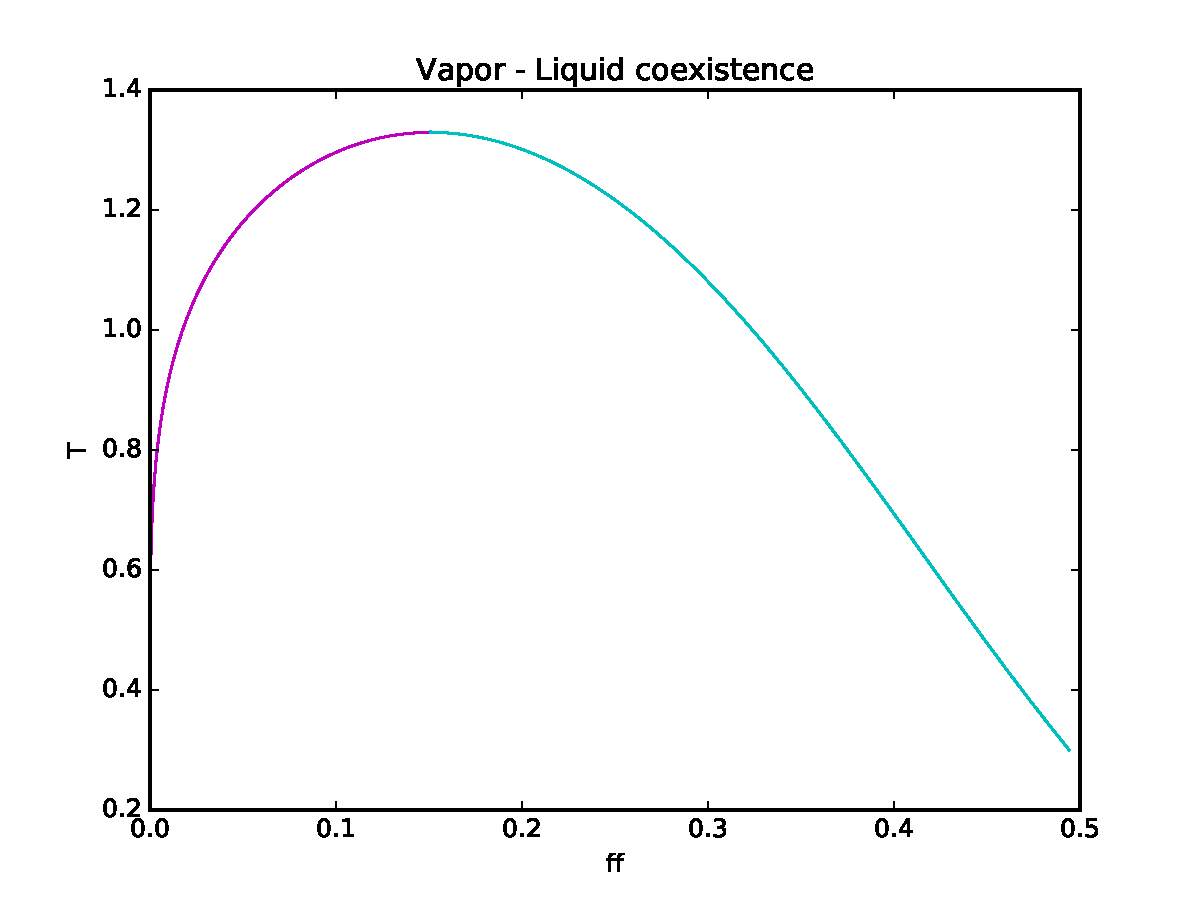
\includegraphics[width=\textwidth]{liqVapCo_Tvsff}
	\caption{Caption 01}
	\label{fig:cap01}
	\end{subfigure}
	\hfill
	\begin{subfigure}[b]{0.3\textwidth}
	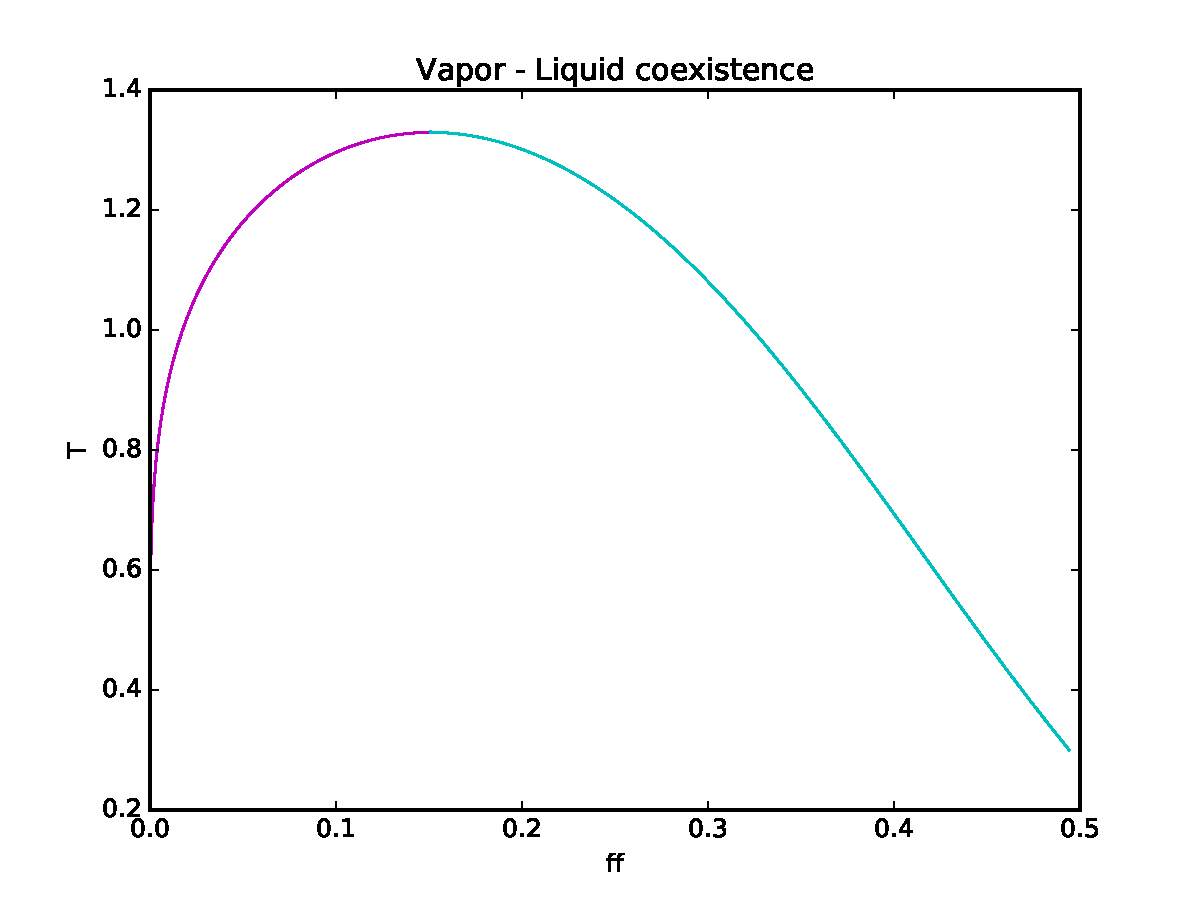
\includegraphics[width=\textwidth]{liqVapCo_Tvsff}
	\caption{Caption 02}
	\label{fig:cap01}
	\end{subfigure}
	\hfill
	\begin{subfigure}[b]{0.3\textwidth}
	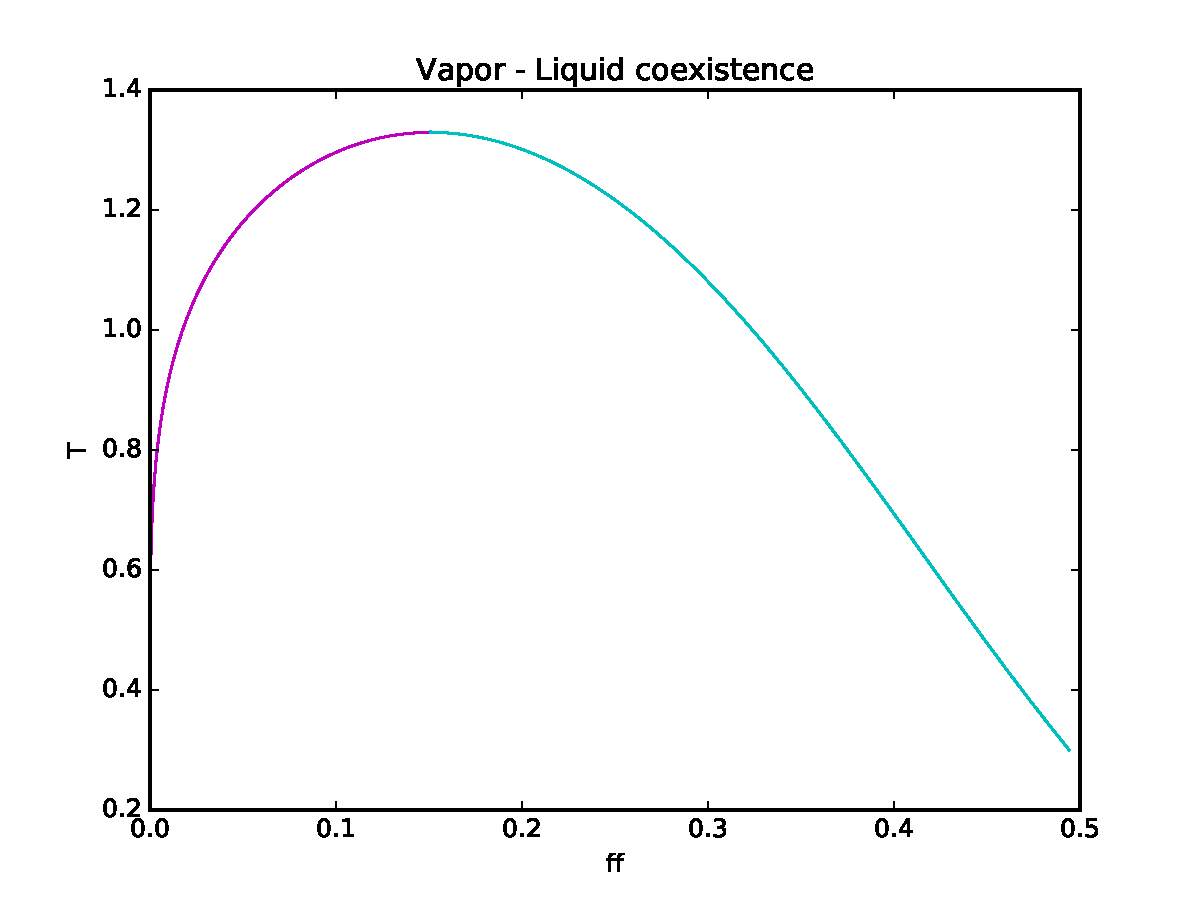
\includegraphics[width=\textwidth]{liqVapCo_Tvsff}
	\caption{Caption 03}
	\label{fig:cap01}
	\end{subfigure}
	\caption{Caption for all three.}
	\label{fig:cap123}
\end{figure}